\documentclass[twoside,openright,11pt]{report}

\usepackage{fullpage}
\usepackage{fancyhdr}
\setlength{\headheight}{15.2pt}
\setlength{\headsep}{10.2pt}
\pagestyle{fancy}

\title{\bf {\Huge Construct}:\\{\LARGE Programming with Geometry}}
\author{{\Large Sam Gruber}\\Carnegie Mellon University}

\lhead{Construct: Programming with Geometry}
\rhead{Sam Gruber}

\setlength{\parskip}{0.5em}

\usepackage{tabularx}
\renewcommand{\arraystretch}{2}

\usepackage{graphicx}

\usepackage{enumerate}

\usepackage{url}

\newcommand{\buttondim}{24pt}

\begin{document}

\maketitle

\chapter{Introduction}
\label{chap:intro}

A programming language is a tool to help the programmer express a solution to a problem.
This tool is most effective when it can clearly translate the intentions of the programmer into the machine's execution process. 
In most modern programming languages, a program is composed of linear sequences of text symbols.
In domains such as text processing or algebraic computation, there is a clear correspondence between this representation of tasks and the way that the programmer imagines them.

However, there are many applications where such a format may not correspond well with the programmer's internal model. 
When the purpose of a program is to manipulate a geometric object, it is a peculiar burden to place upon the programmer to translate the intuitive spatial model of the program into a textual form in order to convey it to a computer. 
A similar disconnect manifests when parallel or concurrent programs are written in a text format that is still fundamentally singular and sequential.

Programmers should have the ability to create programs using tools that can represent the meaning of the program as clearly as possible, rather than having to jump through layers of translation. 
Enabling programming in these ways can open the field to the contributions of less-conventional participants, and could make possible new and different understandings of problems and solutions in computer science.

\section{Goals}
\label{sec:goals}

The target audience for Construct is visual professionals, such as architects and designers, who wish to apply programmatic tools to their existing process.
This audience does not necessarily have experience with modern programming systems, but nonetheless is looking for a way to automate the generation of geometric forms from other geometric forms.
This audience is comfortable thinking about objects in geometric terms, but may not be accustomed to working in symbolic terms.

Construct is designed to bring programming to this audience, where traditional programming often does not correspond to the programmer's mental model.
We target four goals for the design of Construct to help programmers work with the language in a more direct and intuitive way.

\newcommand{\constructgoalsclear}{Make clear the program state}
\newcommand{\constructgoalsnative}{Work in the native representation of geometric relationships}
\newcommand{\constructgoalsnoinfer}{Specify relationships without inference}
\newcommand{\constructgoalscomplete}{Run a full (Turing-complete) range of programs}

\begin{itemize}
  \item {\bf \constructgoalsclear.} 
        The programmer should be able to directly see the state of the program in the programming environment, rather than be required to mentally model the execution of a complex system.
  \item {\bf \constructgoalsnative.} 
        Data and logic which is fundamentally geometric in nature should be expressed geometrically, rather than symbolically. 
        The programmer should not be required to internally translate the meaning of the program to explain it to the computer.
  \item {\bf \constructgoalsnoinfer.} 
        The programmer should be able to clearly and unambiguously present the program to the computer. 
        Inferencing prevents the programmer from clearly understanding what will actually happen when the program runs.
  \item {\bf \constructgoalscomplete.} 
        The medium of programming should not prevent the programmer from expressing any possible program, though it may be better suited to producing certain types of programs.
\end{itemize}

\section{Related Work}
\label{sec:related}

\begin{itemize}
  \item Visual programming with examples tools \cite{victor2013unthinkable}, \cite{victor2013deadfish}
  \item A text-based geometry library with coordinate-free operations and a geometric, rather than algebraic, basis \cite{derose1989coordinatefree}
  \item The Geometric Machine, a model of a computer suited to geometry operations rather than algebraic calculation \cite{reiser2003programming}
\end{itemize}

\chapter{Geometric Syntax}
\label{chap:syntax}

Construct proposes a new geometric method for creating programs. 
Most existing languages offer a textual syntax for composition, which offers an essentially linear approach to writing programs. 
A program in Construct is created by associating geometric objects and relationships in a 2d space. 
This allows the programmer to explore the design of a program in a more open manner, and facilitates the expression of programs which need not have a linear evaluation order. 

Furthermore, a geometric syntax provides a format that can easily express problems which have a geometric or visual interpretation. 
Points, lines, and circles are all primitive objects in Construct, and are presented to the programmer visually, harnessing the brain's highly evolved visual reasoning systems. 

While it is possible to perform symbolic computations in Construct, they are not the target problem set. 
Therefore, a programmer might find certain symbolic tasks, such as text manipulation, as roundabout in Construct as geometric tasks are in a textual syntax.

\section{The Programming Environment}
\label{sec:environ}

Because Construct does not use a textual syntax, programs cannot be composed in a text editor. 
Rather, they require an environment specifically suited to geometric programming. 
This section describes the fundamental characteristics of such an environment and presents a design for its interface.

\begin{figure}[h]
  \centering
  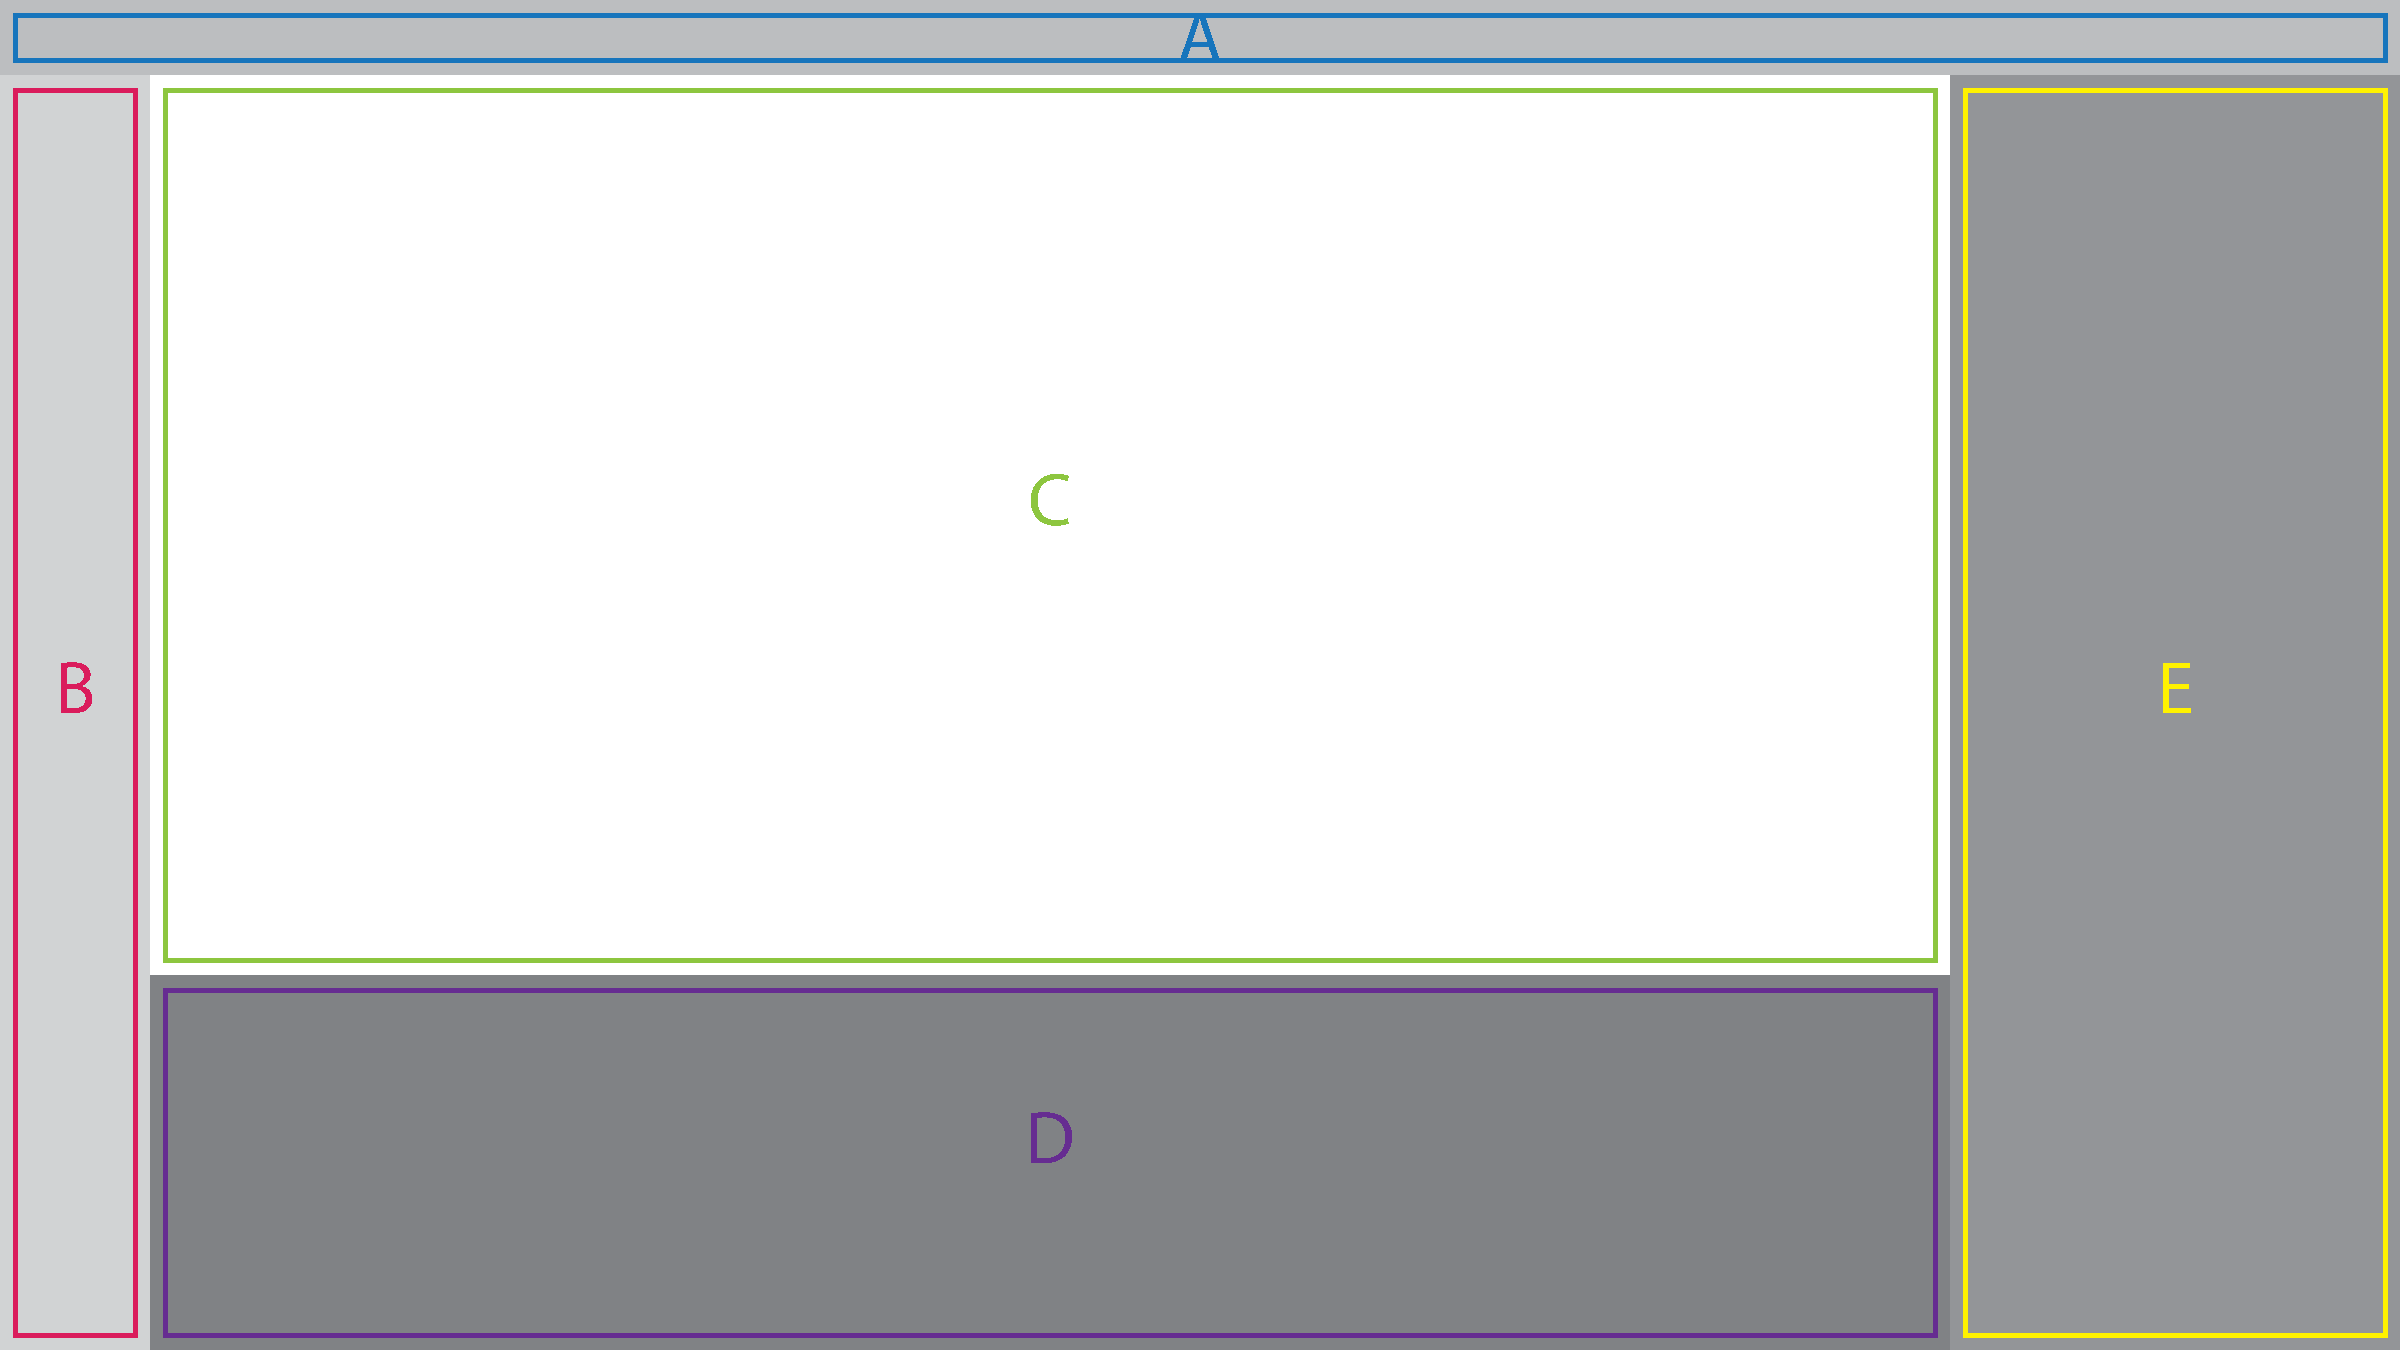
\includegraphics[width=0.9\textwidth]{interface.pdf}
  \caption{An interface design for the programming environment (TODO: detail)}
  \label{fig:interface}
\end{figure}

Figure \ref{fig:interface} shows a general design for the interface, highlighting the five important regions:

\begin{enumerate}[(A)]
  \item Menu Bar \\
    The Menu Bar provides access to functionality which has no representation in the language of the program itself, such as loading or saving programs or starting a live interpreter.
  \item Tool Palettes \\
    Tool Palettes contain commands which create new elements that have meaning in the program. 
    The three main palettes provide commands for Instantiation (see Section \ref{sec:inst}), Definition (see Section \ref{sec:applydef}) and Modification (see Section \ref{sec:applymod}).
  \item Program Space \\
    The Program Space shows a data view of the Construct program. 
    It allows the the programmer to view directly how the program will behave, using representative examples for objects which are not precisely defined. 
    This programming-by-examples approach mimics the manner in which geometry is often taught and worked with, reducing the mental load on the programmer to imagine the meaning of the geometric relationships.
  \item Program Graph \\
    The Program Graph shows the dependency relationships between the objects in Construct. 
    Since all definitions flow from a group of predefined objects to an-as-yet-undefined object, the Program Graph produces a directed acyclic graph (DAG).
  \item User Content Drawers \\
    The User Content Drawers contain definitions which have been created by the programmer as abstractions.
    The programmer may use these definitions in a similar manner to using the built-in definitions.
\end{enumerate}

\section{Object Instantiation}
\label{sec:inst}

To begin working with any of the objects in Construct, the programmer must first {\it instantiate} them. 
One tool palette in the programming environment provides commands that instantiate new objects. 

When first instantiated, a new Construct object is undefined. 
In the case of the point object in Figure \ref{fig:new-point}, this means that it could have any position in the 2d space of the program. 
A line object could have any position and any orientation.
A circle could have any center position and any radius. 
Distances and angles can have any size.

Also notice that the instantiation operation does not require the programmer to name the object. 
In a textual syntax, names are necessary in order for both the programmer and the parser to understand what objects are being used at any stage of the program.
In Construct, the programmer can simply {\it see} the difference between objects.
The system, similarly is free to reference objects directly, since the programming environment can provide an unambiguous description of which objects are being used.
Naming objects is supported in Construct, for the convenience of the programmer, but the names are simply discarded for the purposes of execution.

\section{Applying Definitions}
\label{sec:applydef}

In order for objects to have any meaning, the programmer applies definitions to them. 
These definitions establish relationships between the objects in a Construct program. 
Since definitions are relationships between objects, almost all of them require multiple objects to be instantiated in the program space. 
Section \ref{sec:def} lists the definitions which are built into Construct.

\begin{figure}[h]
  \centering
  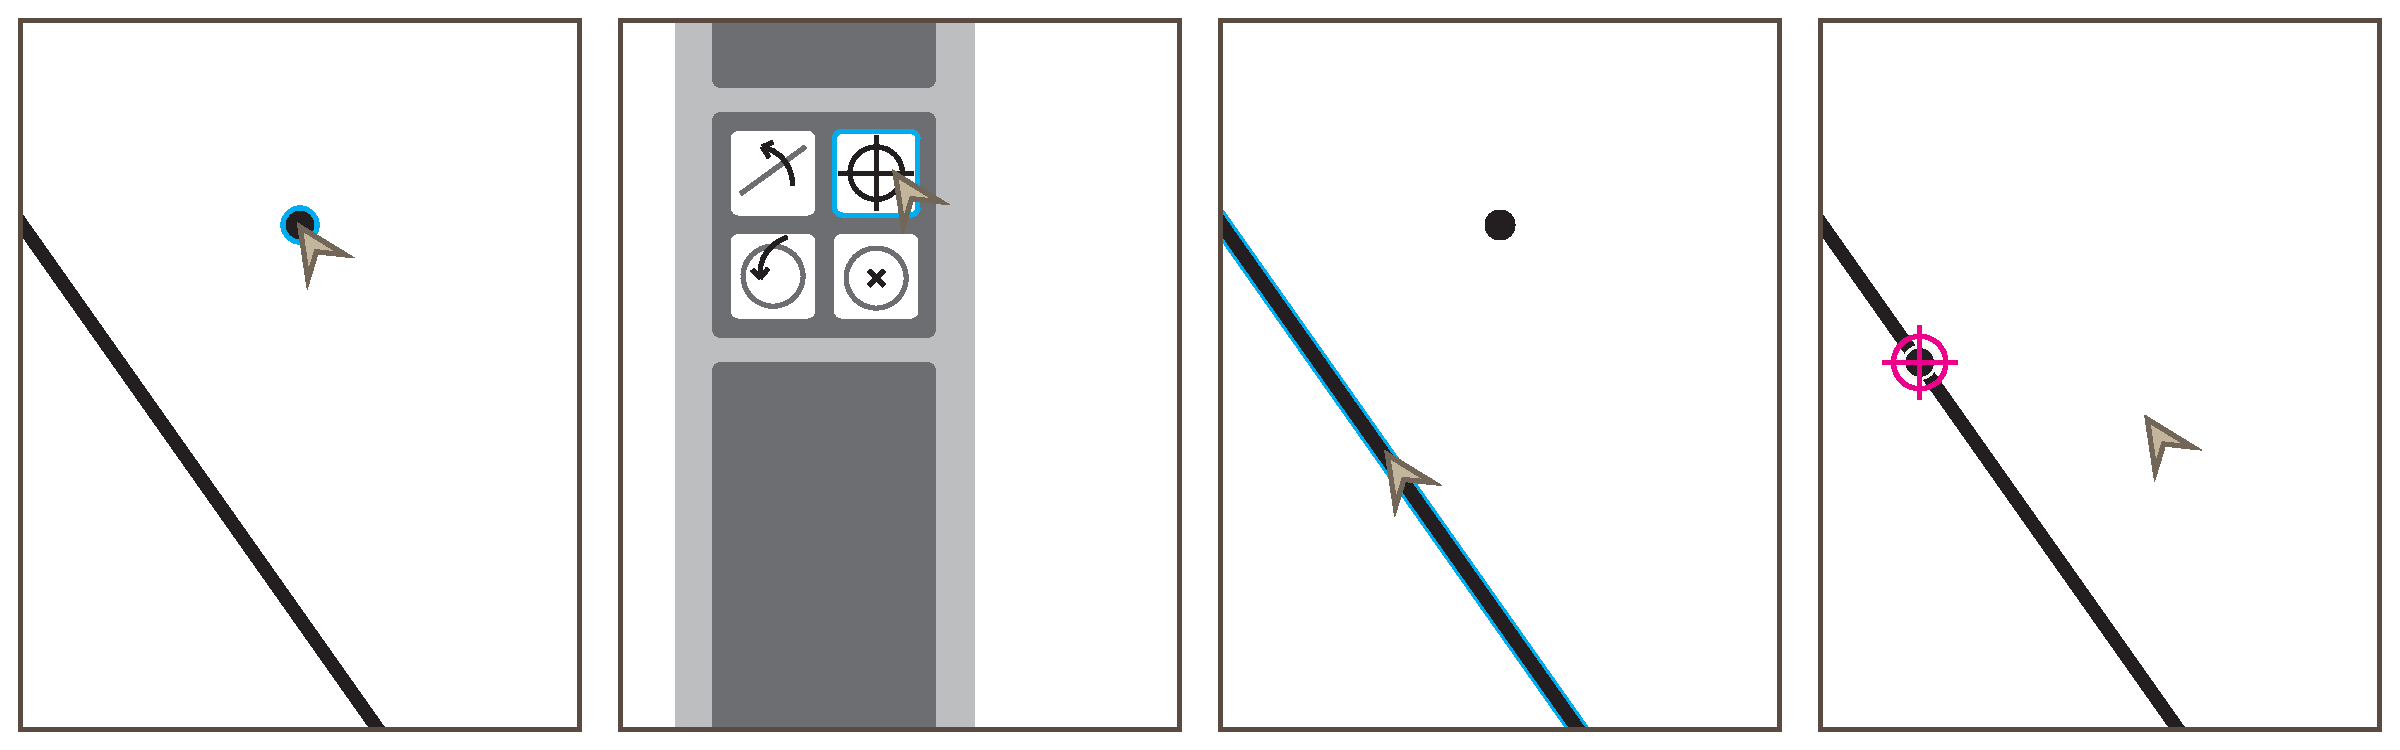
\includegraphics[width=0.9\textwidth]{definition.pdf}
  \caption{The interaction to apply a definition to an object}
  \label{fig:def-interaction}
\end{figure}

Applying a definition is an infix operation in the programming environment. 
First, the programmer selects the object which will be defined. 
Then, the programmer selects a definition from a tool palette in the programming environment. 
Finally, the programmer selects the objects which are referenced by the definition.
Figure \ref{fig:def-interaction} shows how these interactions may appear in the programming environment, using the $\mathsf{on}$ definition as an example.

We can imagine a similar statement in a textual language:

\begin{verbatim}
    Point x = arbitrary_on_line(l);
\end{verbatim}

The effect at runtime of executing this part of the program may not be as linear as the textual equivalent suggests.
In most cases, the object which is being defined will be updated to conform to the new definition's requirements, and other data (if not dependent on the object being defined) will not change.

However, in some cases, the new definition constrains the object in a way that is unsatisfiable. 
In these circumstances, the rest of the program will be recalculated in an attempt to satisfy the new definition. 
If this is successful, the programmer may see many objects in the program space rearrange. 
If it is unsuccessful, the programmer will be alerted that the definitions are unsatisfiable.
More information about errors is presented in Section \ref{sec:failure}.

\subsection{Implicit Definitions}
\label{subsec:implicit-def}

Some definitions which are represented explicitly in the internal representation are in fact implicitly applied in the programming environment.
One such definition is the $\mathsf{elem}$ definition used to extract objects from groups. 
In the geometric syntax, there is no need to explicitly break objects out of groups, because they are already visible to the programmer in the data view.

We present such definitions alongside the others for completeness in Chapter \ref{chap:struct}.
They preserve the uniformity of the internal representation, and are therefore valuable to implementers of the Construct programming environment and interpreter.

\section{Applying Modifications}
\label{sec:applymod}

\subsection{Object Modifications}
\label{subsec:mod-obj}

The process of applying object modifications (Section \ref{subsec:mods-obj}) is quite similar to that of applying definitions.
The programmer first selects the object to be modified, and then selects the modification from a tool palette.

\subsection{Definition Modifications}
\label{subsec:mod-def}

The interactions for definitions modifications vary by modification.
Each of them are outlined below:

\subsubsection{$\mathsf{not}$ Modification}

There are two circumstances when the $\mathsf{not}$ modification can be applied. 
If the programmer wishes to negate a definition which is currently being applied, then after selecting the definition from the appropriate tool palette, the programmer may select $\mathsf{not}$ from its tool palette.
When the definition application is made, it will be negated.

If the programmer wishes to negate a definition which has already been applied to an object, the process is similar to the application of object modifications.
The programmer first selects the definition, and then selects $\mathsf{not}$ from its tool palette.

\subsubsection{$\mathsf{handle}$ Modification}

$\mathsf{handle}$ requires an existing definition to be defined for the object $\rho$. 
The programmer selects this definition, then selects the $\mathsf{handle}$ modifier from its tool palette.
The programmer must then select another definition to serve as the ``failure'' case of the $\mathsf{handle}$. 
This definition is automatically applied to $\rho$. 
The programmer must specify reference objects for the definition as in normal definition application.

\subsubsection{$\mathsf{each}$ Modification}

The $\mathsf{each}$ modification must be specified during the initial definition application process.
First, the programmer selects the object to be defined as normal. 
This object must have type $\mathsf{set}(\tau)$.
Then the programmer activates the $\mathsf{each}$ command from a tool palette, and then selects some definition $\delta_\tau$ appropriate to an object of type $\tau$.
Finally, the reference object must be of type $\mathsf{set}(\tau')$, where $\tau'$ is the type of the reference object for $\delta_\tau$.

\subsubsection{$\mathsf{filter}$ Modification}

The interaction to apply a $\mathsf{filter}$ modification is identical to that of $\mathsf{each}.$

\section{Creating Local Definitions}
\label{sec:create-local}

Local definitions (see Section \ref{sec:local}) allow the programmer to wrap up complex derivations of objects into a single definition without making that internal logic available to other programs.
They are similar to anonymous functions in traditional text-based languages.

\begin{figure}[h]
  \centering
  \fbox{
    \begin{minipage}{3in}\hfill\vspace{2in}\end{minipage}
  }
  \fbox{
    \begin{minipage}{3in}\hfill\vspace{2in}\end{minipage}
  }
  \caption{The appearance of a local definition in the program graph (left) and space (right)}
  \label{fig:local}
\end{figure}

Local definitions can be created from the beginning in a manner similar to the method of applying definitions.
The programmer selects the object to define, then selects the $\mathsf{local}$ tool palette command. 
Unlike a predefined definition, the local definition has no references already defined.

The program space and graph will then appear similar to what is shown in Figure \ref{fig:local}. 
The object which is to be defined will appear locally, marked as $\mathsf{final}$. 
The programmer may then build up the objects and definitions used to define the final object.
If the programmer references an object outside the local definition (distinguishable by the gray overlay that fades those objects), that object will automatically become a reference for the local definition and appear as an $\mathsf{initial}$ inside the local definition.

\section{Definition, Not Manipulation}
\label{sec:not-manip}

It is important to understand that while the Construct programming environment appears in many ways similar to a vector graphics editor, it does not operate by direct manipulation of objects.
The nature of the objects in the program space is given by definition rules which establish relationships between the objects. 
Actually dragging or otherwise transforming the particular objects shown in the program space, while potentially supported for clarification purposes, will have no effect on the meaning of a Construct program.

The program space is presented to the programmer to provide an example of the data in the program at runtime, lifting the burden of mental simulation of the effects of the code. 
Construct is therefore not a programming by example\cite{smith1975pygmalion} system, but rather {\it programming with examples}\cite{myers1986taxonomy}.


\chapter{The Structure of Programs}
\label{chap:struct}

A program in Construct is a Definition (see Section~\ref{sec:def}) which follows a well-defined procedure to generate {\it final} objects from {\it initial} objects. 
Since a program is a Definition, it can used in other programs to abstract away higher-level operations used for generating more complex objects.

A program is a tuple:

$$(O, D, M_\rho, M_\delta)$$

$O$ is the set of all objects (see Section \ref{sec:obj}) that are present in the program. 
$D$ is a function $\rho \to \{\delta_1, \delta_2, \dots\}$ which, given an object $\rho$, produces the set of all definitions (see Section \ref{sec:def}) which describe $\rho$.
$M_\rho$ is a function $\rho \to \{\mu_1, \mu_2, \dots\}$ which, given an object $\rho$, produces the set of all modifiers (See Section \ref{subsec:mods-obj}) which describe $\rho$.
$M_\delta$ is a function $\delta \to \{\mu_1, \mu_2, \dots\}$ which, given an object $\rho$, produces the set of all modifiers (See Section \ref{subsec:mods-defs}) which describe $\delta$.

$O$ and $D$ may be combined to generate a directed acyclic graph $G$. 
Any valid topological sorting of $G$ is a valid ordering of runtime execution for the program.

\section{Objects}
\label{sec:obj}

An object in Construct is an entity $\rho$ which exists in 2d space. 
Objects may have position, orientation, magnitude, or any other characteristics which are appropriate based upon their Type (see Section \ref{sec:types}). 

Objects may be named by user-provided strings. 
These names will appear in the programming environment to disambiguate objects in complex algorithms.
However, since the visual display of Construct disambiguates objects in a manner not possible in a text language, naming of objects is not necessary in simple programs.
There are no restrictions on the format of object names (or even their reuse), as the environment does not rely on names to identify objects.

At any point in the execution of a Construct program, any object is a representative of the {\it valid parameter set}. 
This is a set which contains all parameter combinations which are valid based upon the Definitions (see Section \ref{sec:def}) of the object.

\section{Types}
\label{sec:types}

Construct is strongly typed and does not support parametric typing in any user-created definitions. 
Typing in Construct may also be considered explicit, by nature of the live data representation of the program state. 
The types available in Construct are listed below: \\

\noindent\begin{tabularx}{\textwidth}{l l l c X}
$\tau$ & $::=$ & $\mathsf{pt}$ & \raisebox{-.5\height}{\includegraphics[width=\buttondim]{buttons/pt}} & A point in 2d space. \\
 & & $\mathsf{ln}$ & \raisebox{-.5\height}{\includegraphics[width=\buttondim]{buttons/ln}} & An infinite line in 2d space. \\
 & & $\mathsf{circ}$ & \raisebox{-.5\height}{\includegraphics[width=\buttondim]{buttons/circ}} & A circle in 2d space. \\
 & & $\mathsf{ang}$ & \raisebox{-.5\height}{\includegraphics[width=\buttondim]{buttons/ang}} & An angle in 2d space. \\
 & & $\mathsf{dist}$ & \raisebox{-.5\height}{\includegraphics[width=\buttondim]{buttons/dist}} & A distance in 2d space. \\
 & & $\mathsf{set}(\tau)$ & \raisebox{-.5\height}{\includegraphics[width=\buttondim]{buttons/set}} & A homogeneous collection of objects of type $\tau$. \\
 & & $\mathsf{grp}(\tau_1, \dots, \tau_n)$ & \raisebox{-.5\height}{\includegraphics[width=\buttondim]{buttons/grp}} & A ordered collection of objects.
\end{tabularx}

We can further distinguish the types of objects into three kinds. 
$\mathsf{pt}$, $\mathsf{ln}$ and $\mathsf{circ}$ are {\it literals}, because they correspond to real objects. 
$\mathsf{ang}$ and $\mathsf{dist}$ are {\it measures}. 
They correspond to familiar geometric concepts, but don't have actual position in the real world, and so behave somewhat differently in the program space. 
Finally, $\mathsf{set}$ and $\mathsf{grp}$ are {\it aggregates}, which hold multiple other objects, allowing for complex data structures.

Additionally, some built-in Definitions (see Section \ref{sec:def}) accept numerals as parameters. 
Numerals are shown here with a bar, for example $\bar{n}$ is some integer $n$.
These numerals allow convenient specification of constant values. 
Programmer-created definitions can not accept numerals as inputs. 

Because Construct is inherently connected to a graphical editing environment, each type listed above is associated with an iconic representation of its data.
In the programming environment (see Section \ref{sec:environ}), these icons are displayed in tool palettes and denote the commands used to instantiate new objects of the corresponding type.

The icons shown above were chosen to relate to the programmer's existing vocabulary of geometric objects, and to be visually distinctive from each other. 
For example, we can consider the icons for $\mathsf{set}$ and $\mathsf{grp}$: Because sets are homogeneous and unordered, the icon shows an unorganized cluster of identical triangles. 
By contrast, since groups are both heterogeneous and ordered, the icon shows a line, circle and triangle, arranged linearly.

\section{Definitions}
\label{sec:def}

Definitions are rules that are used to describe an object based upon other objects. 
All of an object's definitions are evaluated at runtime, during Reconciliation (see Section~\ref{sec:reconc}). 

Each Definition is a member of a Definition Class $\delta_\tau$, which is the class of all Definitions that describe objects of type $\tau$. 
Each Definition's inputs and outputs must be a single object, though groups and sets may be passed.
A Definition may be totally described in this notation (group syntax simplified for brevity): 

$$\mathsf{defname}[\tau](\rho_1 : \tau_1; \rho_2 : \tau_2; \dots)$$

If the Definition is listed as part of a Definition Class (as below), we omit the bracketed type information for brevity. 
Additionally, we do not specify the type in our syntax (see Chapter \ref{chap:howto}) because it can be derived from context.

Definition icons, like type icons, appear in the tool palettes of the programming interface. 
They also appear in the program graph as annotations to the edges in the graph, in order to quickly explain the relationships between objects in the program.

\subsection{Generic Definitions}
\label{subsec:def-gen}

The following Definitions describe objects of any type $\tau$. \\

\noindent\begin{tabularx}{\textwidth}{p{0.5cm} p{0.5cm} p{5cm} c X}
$\delta_{\tau}$ & $::=$ & $\mathsf{null}$ & \raisebox{-.5\height}{\includegraphics[width=\buttondim]{buttons/null}} & This definition has no effect on this object. It may be used with the $\mathsf{handle}$ modifier (see Section \ref{subsec:mods-defs}). \\
 & & $\mathsf{id}(\rho : \tau)$ & \raisebox{-.5\height}{\includegraphics[width=\buttondim]{buttons/id}} & This object is identical to $\rho$. \\
 & & $\mathsf{of}(s : \mathsf{set}(\mathsf{\tau}))$ & \raisebox{-.5\height}{\includegraphics[width=\buttondim]{buttons/of}} & This object is identical to a member of the set $s$. This definition is added implicitly in the programming environment when the user manipulates a set member. \\
 & & $\mathsf{elem}(\bar{m}; \; g : \mathsf{group}(\tau_1, \dots, \tau_n))$ & [impl] & This object is the $m$th object in the group $g$. If $m > n$ or $\tau_m \neq \tau$, raise $\mathsf{DefErr}$. This definition is added implicitly in the programming environment when the user manipulates an object inside a group.
\end{tabularx}

The icons that represent these definitions were again chosen to align with symbols familiar to the programmer.
The icon for $\mathsf{null}$ bas been chosen to resemble the common slashed-circle negation symbol, though special attention was paid to create an icon which is visibly distinct from the similar icons for $\mathsf{cross}$ (see Section \ref{subsec:def-ln}).

The $\mathsf{id}$ icon was chosen to resemble the mathematical equivalence operator $\equiv$, rather than the more common equality symbol $=$ because the latter symbol could be easily confused with the usual symbol for parallel lines, used by $\mathsf{par}$ (see Section \ref{subsec:def-ln}).

The $\mathsf{of}$ symbol, as the extraction device for sets, has an icon very similar to the $\mathsf{set}$ type shown in Section \ref{sec:types}.
A single member of the set is distinguished in the $\mathsf{of}$ icon to call attention to its purpose.

One definition listed here, $\mathsf{elem}$, does not have an iconic representation. 
This is because both in the program space and program graph, using an element of a tuple is most clearly presented as an implicit operation to the programmer. 
This definition exists only in the internals of the language and is never exposed to the programmer, and so does not require an iconic representation. 

\subsection{Definitions for $\mathsf{pt}$ Objects}
\label{subsec:def-pt}

\noindent\begin{tabularx}{\textwidth}{p{0.5cm} p{0.5cm} p{5cm} c X}
$\delta_{\mathsf{pt}}$ & $::=$ & $\mathsf{on}(l : \mathsf{ln})$ & \raisebox{-.5\height}{\includegraphics[width=\buttondim]{buttons/on}} & This point occurs somewhere along $l$. \\
 & & $\mathsf{on}(c : \mathsf{circ})$ & \raisebox{-.5\height}{\includegraphics[width=\buttondim]{buttons/on}} & This point occurs somewhere along $c$. \\
 & & $\mathsf{opp}(p : \mathsf{pt}; \; l : \mathsf{ln})$ & \raisebox{-.5\height}{\includegraphics[width=\buttondim]{buttons/opp}} & This point exists on the opposite side of $l$ from $p$. \\
 & & $\mathsf{inside}(c : \mathsf{circ})$ & \raisebox{-.5\height}{\includegraphics[width=\buttondim]{buttons/inside}} & This point occurs inside of $c$. \\
 & & $\mathsf{center}(c : \mathsf{circ})$ & \raisebox{-.5\height}{\includegraphics[width=\buttondim]{buttons/center}} & This point is at the center-point of $c$. \\
 & & $\mathsf{to}(p : \mathsf{pt}; \; d : \mathsf{dist})$ & \raisebox{-.5\height}{\includegraphics[width=\buttondim]{buttons/to}} & This point is at distance $d$ from $p$. \\
 & & $\mathsf{to}(l : \mathsf{ln}; \; d : \mathsf{dist})$ & \raisebox{-.5\height}{\includegraphics[width=\buttondim]{buttons/to}} & This point is at distance $d$ from the nearest location on $l$. \\
 & & $\mathsf{to}(c : \mathsf{circ}; \; d : \mathsf{dist})$ & \raisebox{-.5\height}{\includegraphics[width=\buttondim]{buttons/to}} & This point is at distance $d$ from the nearest location on the circumference of circle $c$. \\
\end{tabularx}

Here we see that the built-in definitions may be overloaded to apply to different combinations of arguments. 
When this is done, the icons for the definitions do not change, in order to minimize the number of icons that are shown in the tool palettes. 
Definitions which are overloaded always describe logically similar relations between objects.

For example, the $\mathsf{on}$ definition is overloaded because a point can be on a line or on a circle. 
To require the programmer to think about which object type the point is on is an excessive burden that does not align with how such relationships are ordinarily discussed in geometry. 
Though the internal calculations will be different, Construct exposes a logically consistent interface to the programmer which allows such details to be handled transparently by the language.

The $\mathsf{on}$ definition is represented by a reticule icon to disambiguate it from several symbols which may appear similar. 
$\times$ or $+$ are commonly used to indicate point objects in graphics editing programs; however, these symbols can potentially be confused with the symbols for intersection (see $\mathsf{intr}$ in Section \ref{subsec:def-ln}). 
Therefore, the reticule symbol has been chosen to refer to the alignment of a point to another object. 
The circle component of the reticule has been reduced in size to likewise avoid confusion with the icon for the $\mathsf{center}$ definition.

To represent $\mathsf{opp}$ and $\mathsf{inside}$, an curved arrow is shown pointing to the zone in which the point is intended to occur. 
The curvature of the arrow reinforces the sense of the line or circle as a boundary applied to the object (which is then being ``leapt over'').
Additionally, the icon avoids a straight arrow to avoid the assumption of a distance or direction relation to the referenced objects.

The $\mathsf{center}$ definition does make use of a traditional locus symbol, since there is no possibility of confusion with any of the other symbols presented to the user, due to the surrounding circle.

There were several challenges to the design of the $\mathsf{to}$ definition icon. 
1) $\mathsf{to}$ will be a highly overloaded definition, having to accommodate all of the possible combinations of input and output objects; 2) the icon should be visually distinct from the icon representing the $\mathsf{dist}$ type; and 3) the icon should not suggest directionality because distances in Construct are scalar.
Therefore, the $\mathsf{to}$ icon shows a point and a line, with a spanning line segment that represents the distance between. 
The gaps between the objects and the distance are similar to gaps left in traditional architectural dimensioning notation.

\subsection{Definitions for $\mathsf{ln}$ Objects}
\label{subsec:def-ln}

\noindent\begin{tabularx}{\textwidth}{p{0.5cm} p{0.5cm} p{5cm} c X}
$\delta_{\mathsf{ln}}$ & $::=$ & $\mathsf{thru}(p : \mathsf{pt})$ & \raisebox{-.5\height}{\includegraphics[width=\buttondim]{buttons/thru}} & This line passes through $p$. \\
 & & $\mathsf{intr}(l : \mathsf{ln})$ & \raisebox{-.5\height}{\includegraphics[width=\buttondim]{buttons/intr}} & This line intersects $l$ at some location. \\
 & & $\mathsf{par}(l : \mathsf{ln})$ & \raisebox{-.5\height}{\includegraphics[width=\buttondim]{buttons/par}} & This line is parallel to $l$. \\
 & & $\mathsf{perp}(l : \mathsf{ln})$ & \raisebox{-.5\height}{\includegraphics[width=\buttondim]{buttons/perp}} & This line is perpendicular to $l$. \\
 & & $\mathsf{skew}(a : \mathsf{ang}; \; l : \mathsf{ln})$ & \raisebox{-.5\height}{\includegraphics[width=\buttondim]{buttons/skew}} & This line is at angle $a$ to line $l$. \\
 & & $\mathsf{tan}(c : \mathsf{circ})$ & \raisebox{-.5\height}{\includegraphics[width=\buttondim]{buttons/tan}} & This line has a point of tangency to $c$ at some location. \\
 & & $\mathsf{cross}(c : \mathsf{circ})$ & \raisebox{-.5\height}{\includegraphics[width=\buttondim]{buttons/cross}} & This line intersects $c$ at two locations. \\
 & & $\mathsf{to}(p : \mathsf{pt}; \; d : \mathsf{dist})$ & \raisebox{-.5\height}{\includegraphics[width=\buttondim]{buttons/to}} & This line is at distance $d$ from point $p$ at it closest location. \\
 & & $\mathsf{to}(l : \mathsf{ln}; \; d : \mathsf{dist})$ & \raisebox{-.5\height}{\includegraphics[width=\buttondim]{buttons/to}} & This line is at distance $d$ to line $l$ at their closest points. In two dimensions, this implies $\mathsf{par}(l)$. \\
 & & $\mathsf{to}(c : \mathsf{circ}; \; d : \mathsf{dist})$ & \raisebox{-.5\height}{\includegraphics[width=\buttondim]{buttons/to}} & This line is at distance $d$ from the nearest location on the circumference of circle $c$. \\
\end{tabularx}

\subsection{Definitions for $\mathsf{circ}$ Objects}
\label{subsec:def-circ}

\noindent\begin{tabularx}{\textwidth}{p{0.5cm} p{0.5cm} p{5cm} c X}
$\delta_{\mathsf{circ}}$ & $::=$ & $\mathsf{thru}(p : \mathsf{pt})$ & \raisebox{-.5\height}{\includegraphics[width=\buttondim]{buttons/thru}} & This circle passes through $p$. \\
 & & $\mathsf{about}(p : \mathsf{circ})$ & \raisebox{-.5\height}{\includegraphics[width=\buttondim]{buttons/center}} & This circle is centered on $p$. \\
 & & $\mathsf{tan}(l : \mathsf{ln})$ & \raisebox{-.5\height}{\includegraphics[width=\buttondim]{buttons/tan}} & This circle has a point of tangency to $l$ at some location. \\
 & & $\mathsf{tan}(c : \mathsf{circ})$ & \raisebox{-.5\height}{\includegraphics[width=\buttondim]{buttons/tan}} & This circle has a point of tangency to $c$ at some location. \\
 & & $\mathsf{cross}(l : \mathsf{ln})$ & \raisebox{-.5\height}{\includegraphics[width=\buttondim]{buttons/cross}} & This circle intersects $l$ at two locations. \\
 & & $\mathsf{to}(p : \mathsf{pt}; \; d : \mathsf{dist})$ & \raisebox{-.5\height}{\includegraphics[width=\buttondim]{buttons/to}} & This circle's circumference is at distance $d$ from point $p$ at it closest location. \\
 & & $\mathsf{to}(l : \mathsf{ln}; \; d : \mathsf{dist})$ & \raisebox{-.5\height}{\includegraphics[width=\buttondim]{buttons/to}} & This circle's circumference is at distance $d$ to line $l$ at their closest points. \\
 & & $\mathsf{to}(c : \mathsf{circ}; \; d : \mathsf{dist})$ & \raisebox{-.5\height}{\includegraphics[width=\buttondim]{buttons/to}} & This circle's circumference is at distance $d$ from the nearest location on the circumference of circle $c$. \\
\end{tabularx}

\subsection{Definitions for $\mathsf{ang}$ Objects}
\label{subsec:def-ang}

\noindent\begin{tabularx}{\textwidth}{p{0.5cm} p{0.5cm} p{5cm} c X}
$\delta_{\mathsf{ang}}$ & $::=$ & $\mathsf{join}(a : \mathsf{ang}; \; b : \mathsf{ang})$ & \raisebox{-.5\height}{\includegraphics[width=\buttondim]{buttons/join}} & This angle's sweep is equal to the sum of the sweeps of $a$ and $b$. \\
 & & $\mathsf{split}(a : \mathsf{ang}; \; \bar{n})$ &  & This angle's sweep is equal to $\frac{1}{n}$ times the sweep of $a$. If $n = 0$, raise $\mathsf{DefErr}$. \\
 & & $\mathsf{sweep}(\bar{n})$ & \raisebox{-.5\height}{\includegraphics[width=\buttondim]{buttons/sweep}} & The sweep of this angle is equal to $n$ (in degrees). \\
 & & $\mathsf{between}(k : \mathsf{ln}; \; l : \mathsf{ln}; \; p : \mathsf{pt})$ & \raisebox{-.5\height}{\includegraphics[width=\buttondim]{buttons/skew}} & This angle's sweep is the sweep between the lines $k$ and $l$ which contains $p$. \\
\end{tabularx}

\subsection{Definitions for $\mathsf{dist}$ Objects}
\label{subsec:def-dist}

\noindent\begin{tabularx}{\textwidth}{p{0.5cm} p{0.5cm} p{5cm} c X}
$\delta_{\mathsf{dist}}$ & $::=$ & $\mathsf{sum}(d : \mathsf{dist}; \; t : \mathsf{dist})$ &  & This distance is equal to the sum of the lengths of $d$ and $t$. \\
 & & $\mathsf{div}(d : \mathsf{dist}; \; \bar{n})$ &  & This distance is equal to $\frac{1}{n}$ times the length of $d$. If $n = 0$, raise $\mathsf{DefErr}$. \\
 & & $\mathsf{length}(\bar{n})$ & \raisebox{-.5\height}{\includegraphics[width=\buttondim]{buttons/length}} & This distance is equal to $n$.\\
 & & $\mathsf{span}(p : \mathsf{pt}; \; q : \mathsf{pt})$ & \raisebox{-.5\height}{\includegraphics[width=\buttondim]{buttons/to}} & This distance is equal to the distance from $p$ to $q$. \\
 & & $\mathsf{span}(p : \mathsf{pt}; \; l : \mathsf{ln})$ & \raisebox{-.5\height}{\includegraphics[width=\buttondim]{buttons/to}} & This distance is equal to the shortest distance from $p$ to $l$. \\
 & & $\mathsf{span}(p : \mathsf{pt}; \; c : \mathsf{circ})$ & \raisebox{-.5\height}{\includegraphics[width=\buttondim]{buttons/to}} & This distance is equal to the shortest distance from $p$ to $c$. \\
 & & $\mathsf{span}(k : \mathsf{ln}; \; l : \mathsf{ln})$ & \raisebox{-.5\height}{\includegraphics[width=\buttondim]{buttons/to}} & This distance is equal to the shortest distance from $k$ to $l$. \\
 & & $\mathsf{span}(l : \mathsf{ln}; \; c : \mathsf{circ})$ & \raisebox{-.5\height}{\includegraphics[width=\buttondim]{buttons/to}} & This distance is equal to the shortest distance from $l$ to $c$. \\
 & & $\mathsf{span}(b : \mathsf{circ}; \; c : \mathsf{circ})$ & \raisebox{-.5\height}{\includegraphics[width=\buttondim]{buttons/to}} & This distance is equal to the shortest distance from $b$ to $c$. \\

\end{tabularx}

\subsection{Definitions for $\mathsf{set}(\tau)$ Objects}
\label{subsec:def-set}

\noindent\begin{tabularx}{\textwidth}{p{0.5cm} p{0.5cm} p{5cm} c X}
$\delta_{\mathsf{set}}$ & $::=$ & $\mathsf{empty}$ &  & This set has no members. \\
 & & $\mathsf{size}(\bar{n})$ &  & The number of members of this set. \\
 & & $\mathsf{include}(\rho : \tau; s : \mathsf{set}(\tau))$ &  & This set contains all members of the set $s$ and additionally contains $\rho$. \\
 & & $\mathsf{exclude}(\rho : \tau; s : \mathsf{set}(\tau))$ &  & This set contains all members of the set $s$ except $\rho$. If $\rho$ is not a member of $s$, raise $\mathsf{DefErr}$.
\end{tabularx}

\subsection{Definitions for $\mathsf{grp}(\tau_1, \dots , \tau_n)$ Objects}
\label{subsec:def-grp}

\noindent\begin{tabularx}{\textwidth}{p{0.5cm} p{0.5cm} p{5cm} c X}
$\delta_{\mathsf{grp}}$ & $::=$ & $\mathsf{collect}(\rho_1 : \tau_1, \dots, \rho_n : \tau_n)$ & [impl] & This group contains $\rho_1, \dots, \rho_n$.
\end{tabularx}

Like the $\mathsf{elem}$ definition (see Section \ref{subsec:def-gen}), $\mathsf{collect}$ need not be explicitly available in the programming environment. 
Groups are constructed by the group typing tool and visually marked as combined objects in the program space and program graph. 
This definition is used internally by the implementation.

\section{Modifiers}
\label{sec:mods}

Modifiers are higher-level constructs than Definitions which further specify program behavior.

\subsection{Modifiers for Objects}
\label{subsec:mods-obj}

\noindent\begin{tabularx}{\textwidth}{p{0.5cm} p{0.5cm} p{5cm} c X}
$\mu_{\rho}$ & $::=$ & $\mathsf{initial}$ &  & $\rho$ is given as an input to the program. \\
 & & $\mathsf{final}$ &  & $\rho$ is the result of the program. \\
 & & $\mathsf{unique}$ &  & The Definitions which specify $\rho$ must resolve to exactly one possible set of parameters. If $\rho$ is not uniquely defined, raise $\mathsf{DefErr}$.
\end{tabularx}

\subsection{Modifiers for Definitions}
\label{subsec:mods-defs}

\noindent\begin{tabularx}{\textwidth}{p{0.5cm} p{0.5cm} p{5cm} c X}
$\mu_{\delta_\tau}$ & $::=$ & $\mathsf{not}$ &  & The negation of this Definition. \\
 & & $\mathsf{handle}(\delta_\tau')$ &  & If this Definition raises a runtime error, instead apply $\delta_\tau'$. \\
 & & $\mathsf{each}$ &  & Applies this Definition over all members of a set, specifying a new Definition in the class $\delta_{\mathsf{set}(\tau)}$. If $\mathsf{DefErr}$ is raised at any point, this whole definition raises $\mathsf{DefErr}$. \\
 & & $\mathsf{filter}$ &  & Applies this Definition over all members of a set. If the definition does not raise an error, include its {\it final} object in the new set. Otherwise, skip that object without raising $\mathsf{DefErr}$. \\
\end{tabularx}

\section{Local}
\label{sec:local}
\noindent\begin{tabularx}{\textwidth}{p{0.5cm} p{0.5cm} p{5cm} c X}
$\lambda$ & $::=$ & $\mathsf{local}(G)$ &  & Produces a local definition from the program subgraph $G$. This can be used in conjunction with the $\mathsf{handle}$, $\mathsf{each}$ and $\mathsf{filter}$ modifiers to apply more complex behaviors.\\
\end{tabularx}


\chapter{Execution}
\label{chap:exec}

\section{Runtime Errors}
\label{sec:runtime-errors}

\begin{tabularx}{\textwidth}{l l l X}
$\epsilon$ & $::=$ & $\mathsf{DefErr}$ & A set of Definitions (see Section \ref{sec:def}) could not be Reconciled (see Section \ref{sec:reconc}) to a valid object.
\end{tabularx}

\section{Reconciliation}
\label{sec:reconc}

When an object in the Evaluation DAG becomes definable (when all of its immediate prerequisites are defined), the Construct runtime begins a process of Reconciliation. 
During Reconciliation the runtime attempts to find a state for the object which satisfies all of the Definitions applied to it. 
It selects a candidate object from the set of all objects which satisfy the constraints placed upon it.

\section{Failure}
\label{sec:failure}

During runtime, it is possible for Reconciliation to fail by an object possessing conflicting definitions. 

This may initially occur as a result of choices made during the reconciliation of ancestor objects in the program. 
The runtime will first try to resolve the failure by redefining these ancestors in a way that will produce a valid result. 
If this is unsuccessful, the runtime declares $\mathsf{DefErr}$.

A runtime error is then propagated back along the chain of ancestor definitions from the definition which triggered it. 
If the runtime encounters a definition which has a $\mathsf{handle}$ modifier attached to it, it will stop this propagation and attempt to redefine the program using the alternate definition.
This definition itself may fail, which repeats this process on the changed program graph.

If the runtime error propagates all the way to to the initial objects at the top level of the program, the program has failed. 
The user should be alerted to the failure, and if the program is being evaluated in the programming environment, specific debugging information should be made available.

\chapter{How to Program in Construct}
\label{chap:howto}

In this chapter, we discuss points relevant to prospective programmers in Construct. Common programming idioms are shown, as well as some examples of functionality that can be built using the tools we have described previously.

\section{Idioms}
\label{sec:idioms}

This section shows some common programming idioms in Construct in isolation from their broader context.

\subsection{Natural Numbers}
\label{subsec:nats}

\subsection{Counting Down}
\label{subsec:countdown}

\subsection{If Then Else}
\label{subsec:if}

\section{Example Programs}
\label{sec:example}

Below we show some example programs that can be written using the features of Construct described earlier in this document. 
Each example begins with a view of the program in its final form, showing both the program space with the concluding state of the program, and the program graph of the definition dependencies of the whole program.

\pagebreak

\subsection{Triangle Area}
\label{subsec:triarea}

\begin{figure}[h]
  \centering
  \includegraphics[width=0.8\textwidth]{examples/triarea}
  \caption{A Construct program which finds the area of a triangle formed from three input points using elementary geometric reasoning.}
  \label{fig:triarea}
\end{figure}

Figure \ref{fig:triarea} shows a program which calculates the area of the triangle in both the program space and program graph views.

\subsection{Adjacent Segments}
\label{subsec:adjsegs}

This program demonstrates a verification definition. 
Unlike other definitions which produce a resulting object, this definition just ensures that some relationships are satisfied over its inputs. 
Verifications may be used as part of extracting objects from sets, or as contracts in programs.

Here we use an abbreviated textual syntax for referencing objects in groups. 
{\tt obj[1][2]} references the second item in a group which is the first item of a group object named {\tt obj}. 
This notation is similar to array addressing in modern textual programming languages. \\

\noindent \begin{tabularx}{\textwidth}{l X p{4cm}}
\hspace{3.5cm}\vspace{1cm} & {\tt initial grp(grp(ln;circ);\newline grp(ln;circ)) segs } & {\small Start with two segments (represented by a line and a bounding circle). } \\
\hline
\vspace{0.5cm} & 
{\tt
pt adj.on(segs[1][1]) \newline
      .on(segs[1][2]) \newline
      .on(segs[2][1]) \newline
      .on(segs[2][2])
} & {\small Verify that the lines and circles all intersect at a common point.} \\
\end{tabularx}\\\\

If this simple definition fails, then we know that our line segments are not adjacent.

\subsection{Reduce Polygon to Triangle}
\label{subsec:reducepoly}

TODO

\subsection{Polygon Area}
\label{subsec:polyarea}

The next example program incorporates the previous examples and calls them as user-created definitions. 
We use the keyword {\tt void} to where a verification definition produces no resulting object; in the geometric interface, this is invisible to the programmer.

User-created definitions are enclosed in curly braces to distinguish them from the built-in definitions. 
Local definitions are also enclosed in curly braces, but not named. \\

\noindent \begin{tabularx}{\textwidth}{l X p{4cm}}
\hspace{3.5cm} & {\tt final set(grp(ln;circ)) tri.local\{ \newline
  initial set(grp(ln;circ)) poly.size(3) \newline
  void.\{Closed Polygon\}(poly) \newline
  final poly \newline
\}} & {\small If the polygon has three sides, then it's already a triangle. } \\
\hline
 & {\tt handle( local\{ \newline
  initial set(grp(ln;circ)) poly \newline
  void.\{Closed Polygon\}(poly) \newline
  final poly3.\{Reduce Polygon to \newline Triangle\}(poly) \newline
\})} & {\small If the polygon has more than three sides, we reduce it to three. } \\
\hline
 & {\tt grp(ln;circ) A.of(tri) \newline
        grp(ln;circ) B.of(tri) \newline
        .not id(A) \newline
        grp(ln;circ) C.of(tri) \newline
        .not id(A) \newline
        .not id(B) } & {\small Get the three sides. } \\
\hline
\vspace{1.5cm} & {\tt pt p1.on(A[1]).on(B[1]) \newline
        pt p2.on(A[1]).on(C[1]) \newline
        pt p3.on(B[1]).on(C[1])} & {\small Get the three vertices. } \\
\hline
\vspace{1.5cm} & {\tt grp(pt;pt;pt) verts.collect(p1;p2;p3) \newline
        final dist area.\{Triangle Area\}(verts)} & {\small Use the triangle area definition. } \\
\end{tabularx}\\\\

\chapter{Conclusions}
\label{chap:conclusions}

\section{Future Work}
\label{sec:future}

At this time, Construct exists only as this general specification of a programming system. 
Future work on this system may take many directions, some of which are described below.

\subsection{Runtime Implementation}

This document only describes the behavior of Construct programs. 
It will be necessary to produce a working interpreter or compiler than can enable these programs to be actually written and tested. 
This runtime system will require a constraint solver that can efficiently step the program forward so that Construct is a viable alternative to traditional programming languages.

\subsection{Interface Implementation}

In order to assess the usability of the interface to Construct, future work should explore a prototype of the programming environment described in Chapter \ref{chap:syntax}.
This prototype can then be tested with the target audience of visual professionals to gauge its effectiveness and gain user feedback on the design decisions made in the system.

\subsection{Cut and Paste}

An interface challenge to be explored in future work is the functionality of cut and paste. 
In textual programming languages, cut and paste can be performed independently of the surrounding text because there are no explicit linkages.
Because Construct programs are presented to the programmer as directed graphs, performing cut and paste requires some trade-off between preserving edges (representing definitions), and maintaining predictability of the command to the programmer.

{\bf CITE IBRAHIM}

\subsection{Higher Dimensions}

Presently, Construct has been designed to facilitate geometric procedures solely in a two-dimensional plane. 
This is a significant limitation on the problems which are easily represented by the system. 
While approaches from projective geometry may be used to simulate working in higher dimensions, such approaches require the programmer to mentally simulate the true operation of the program, which falls short of Goal 1 (see Section \ref{sec:goals}).
Extension of the design of Construct to three dimensions in future work could alleviate this problem.

\subsection{Datatypes}

Programmers will likely desire to shorthand complex datatypes composed of sets and groups into single entities. 
Several of the examples presented in Section \ref{sec:example} make use of a group of a line and a circle to represent a line segment. 
In those examples, we must verify that the group is a valid segment, rather than having the language establish this for us.
Future work may explore adding the facility to Construct for arbitrary higher-complexity datatypes to be reduced to simpler programmer-created type definitions.

\section{Discussion}
\label{sec:discuss}

In Section \ref{sec:goals} we laid out four goals to help programmers to use Construct. Each of these principles have shaped the design of this programming system.

\subsection{\constructgoalsclear}

Construct programs are shown to the programmer in an environment (Section \ref{sec:environ}) which displays both a graph of the evaluation of the program and a representative state of its objects.
In this way, the programmer is relieved of the burden of simulating the operation of the program.

\subsection{\constructgoalsnative}

Chapter \ref{chap:struct} describes the many features in Construct which mimic their traditional pen-and-paper geometry counterparts.
All objects in Construct have familiar analogs in geometry and behave in ways that are consistent with traditional geometry.
Likewise, the definitions correspond to common geometric operations, and can be clearly explained using terminology familiar to any user who has worked with geometry.

\subsection{\constructgoalsnoinfer}

Unlike programming by example systems, Construct is designed to be programmed entirely by specifying unambiguous rules.
This prevents the uncertainty of relying on the environment's inference engine, and allows the programmer to be confident in the formulation of the program.

\subsection{\constructgoalscomplete}

\appendix

\nocite{*}

\bibliographystyle{acm}
\bibliography{construct}

\end{document}